\documentclass[../../thesis.tex]{subfiles}

\begin{document}

\TODO{relate our work to TimeVQVAE, Neural Representation, Barlow, MaskGIT, }

\TODO{Include something on time series generation / representation learning}


Our work in this thesis can be seen as a tangent of the paper "Vector Quantized Time Series Generation with a Bidirectional Prior Model" \cite{TimeVQVAE}. The TimeVQVAE model is a two staged process. For this part of the thesis we focused on the first stage (tokenization) of the model. Meaning that we did not fit a prior on the latent space, keeping it uniform. Further we simplified the model by not separating the high and low frequency components of the data.\\\\

To our knowledge the joint embedding VQ-VAE models presented in this thesis are new.

\section{TimeVQVAE}

\section{MaskGIT}

The Masked Generative Image Transformer is a generative transformer model for image synthesis developed by Google Research. The novelty of the model lies in the token generation. Unlike popular autoregressive generative transformers, who treat images as a sequence of tokens, MaskGIT introduces an image synthesis paradigm using a bi-directional transformer decoder. This means that during training MaskGIT learns to predict tokens in all directions, an intuitively more natural way to consider images. At inference time MaskGIT starts out with a blank canvas and predicts the entire image, and iteratively keeps and conditions on the most confident pixels.\\\\

\TODO{Intuitive introduction of masked modelling. Figures and such.}

The model assumes a tokenization procedure for stage 1, and in the original paper they used VQGAN \cite{VQGAN}. As MaskGIT only focuses on improving stage 2, present only that part. 

\subsection{Prior learning}

Start out with a sequence $s$ (b,n) of codebook indeces corresponding to a discrete latent representation $z_q$. Determine the proportion of tokens to mask according to the mask scheduling function $\gamma(t)\in (0,1]$. 
Sample a random subset of $s$ and replace values by [MASK] token in order to create the masked sequence $s_M$ (b,n). By a forward pass of the bi-directional transformer with $s_M$ as input obtain unnormalized logits (b,n,K), defining a distribution over the codebook indeces at each element. Calculate the loss as the binary cross-entropy of the logits and $s$. 

\subsection{Iterative decoding}

The bi-directional transformer could in principle predict all [MASK] tokens and generate a sample in a single pass by simply sampling from the logits obtained from a forward pass of an all masked sequence. However, there are challenges with this approach. In their original article \todo{spør om siteringsstil, og fiks denne setningen} \cite{chang2022maskgit} proposes a novel non-autoregressive decoding method to sythesize samples in a constant number of steps.\\\\

The decoding process goes from $t = 0$ to $T$. To genereate a sample at inference time one starts out with a all masked sequence which we denote by $s_M^{(0)}$. At iteration $t$ the model predicts the probabilities for all the [MASK] tokens, $p(\hat{s}_{ij}^{(t)}|s_M^{(t)})$, in parallell. Then at each masked entry $ij$ we sample a token index based on its predicted distribution.  

\subsection{Masking design}

For image generation, cosine schedulig function proved best across all experiments in the original paper. Start out by selecing just a few 




\section{SSL}


\subsection{BYOL}
\cite{grill2020bootstrap}
Bootstrap Your Own Latents (BYOL) is an early non-contrastive self supervised learning algorithm developed by Google Research in 2020. BYOL was developed for image representation learning and provided a new state of the art for downstream classification accuracy on ImageNet using a linear evaluation with a ResNet-50 architecture. 

How it works:
BYOL uses a joint embedding architecture, one \textit{online} network and a \textit{target} network. Both networks consists of an encoder $f$ and decoder $g$, while the online network too has a predictor $q$. The architecture of the networks are the same, but the target parameters $\zeta$ are exponential moving averages of the online parameters $\theta$. In particular, for a specified target decay rate $\tau\in[0,1]$, the target parameters are updated according to 
\begin{equation}
    \zeta \leftarrow \tau \zeta + (1-\tau)\theta
\end{equation}
after each training step. \\\\

Let $\mathcal{D}$ be the data. As is typical for non contrastice SSL, data augmentations are applied in order to increase robustness of the representations. Let $\mathcal{T}$  and $\mathcal{T'}$ denote the set of augmentations for the online and target network respectively. BYOL samples a data point $x\sim \mathcal{D}$ and two augmentation $t\sim \mathcal{T}$ and $t'\sim \mathcal{T'}$, with whom it creates two views $v = t(x)$ and $v' = t'(x)$. The views maps through their respective branch as follows

\begin{equation}
    x \to t(x) = v \to f_\theta(v) = y_\theta \to g_\theta (y_\theta) = z_\theta \to p_\theta(z_\theta)
\end{equation}
\begin{equation}
    x \to t'(x) = v' \to f_\zeta(v') = y'_\zeta \to g_\zeta (y'_\zeta) = z'_\zeta,
\end{equation}
and both outputs are $l_2$-normalized before their mean squared error is calculated. In other words the outputs are updated as
\begin{equation}
    \bar{p}_\theta(z_\theta) = \frac{p_\theta(z_\theta)}{||p_\theta(z_\theta)||_2}, \quad \bar{z}_\zeta' = \frac{z_\zeta'}{||z_\zeta'||_2},
\end{equation}
before the loss is obtained by 
\begin{equation}
    \mathcal{L}_{\theta,\zeta} = ||\bar{p}_\theta(z_\theta) - \bar{z}_\zeta'||_2^2 = 2-2 \frac{\langle p_\theta(z_\theta), z_\zeta'\rangle}{||p_\theta(z_\theta)||_2\cdot||z_\zeta'||_2}
\end{equation}

The BYOL loss is obtain by symmetrizing $\mathcal{L}_{\theta,\zeta}$. This is done by separately feeding $v'$ into the online network and $v$ into the target network, and calculating $\mathcal{\tilde{L}}_{\theta,\zeta}$ to obtain $\mathcal{L}^{\text{BYOL}}_{\theta,\zeta} = \mathcal{L}_{\theta,\zeta} + \mathcal{\tilde{L}}_{\theta,\zeta}$


\TODO{Figure}




\subsection{Barlow Twins}
What is it?

Barlow Twins is a non-constrastive SSL method based on applying the \textit{redundancy-reduction principle} (or efficient coding hypothesis) \cite{Barlow_origin} from the neroscientist H. Barlow to a pair of identical networks. 

In essence the models encurage representations of similar samples to be similar, while simultaneously reducing the amount of redundancy between the components of the vectors. This is done by producing two distorted views of each sample and embedding these in a vast feature space, in such a way that their cross-correalion is close to the identity. 

How does it work?

Start out with a sample $X$ and creates two augmented (distorted) views $X_1$ and $X_2$. The views are then mapped to a latent space by two identical encoders, giving $Y_1$ and $Y_2$. Then the projector embeds the latent representations in a vast space, giving $Z_1$ and $Z_2$. Finally the similarity of the two embeddings are measured by the empirical cross-corelation.

\TODO{Ask for premission?? to use this or make own}
\begin{figure}[h]
    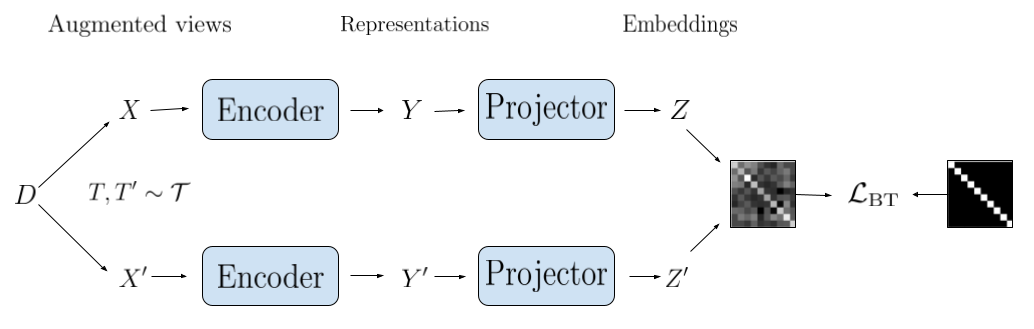
\includegraphics[scale=0.2]{BarlowTwins.png}
    \centering    
    \caption{\cite{zbontar2021barlow}}
\end{figure}

The loss function is calculated as the difference of the empirical cross-correlations of $Z_1$ and $Z_2$ is then calculated and the identiry matrix. 


\subsection{VIbCReg}
\TODO{What is it?}

VIbCReg \cite{lee2024vibcreg} is a non-contrastive SSL model based on VICReg \cite{bardes2022vicreg}, but with better covariance regularization.  It has a joint embedding architecture. 

\TODO{How it works}
Two different views of the input data is encoded into representations $Y$ $Y'$. The representations are further mapped to a larger space by a \textit{projector} with an IterNorm \cite{huang2019iterative} layer. The loss is computed using the projected values $Z$ and $Z'$. \newline
The loss consists of a similarity loss between the branches, and feature decoration (FD) loss together with a feature component expressiveness (FcE) term at each branch. 

\TODO{Loss}
Input data is processed in batches. Denote $Z = [z_1,...,z_B]^T \in \mathbb{R}^{B\times F}$, and similarly for $Z'$, where $B$ and $F$ denotes the batch and feature sizes respectively. $\text{Var}()$ is a variance estimator, $\gamma$ is a target value for the standard deviation, which both in VIbCReg and VICReg is set to $1$. $\epsilon$ is a small scalar preventing numerical instabilities.\newline 
Similarity loss

\begin{equation}
    s(Z,Z') = \frac{1}{B} \sum_{b=1}^B || Z_b-Z_b'||_2^2
\end{equation}

FcE/Variance term

\begin{equation}
    v(z) =  \frac{1}{F} \sum_{f=1}^F \max(0,\gamma - \sqrt{\text{Var}(Z_f)+\epsilon})
\end{equation}


FD/covariance term

\begin{equation}
    C(Z) = \frac{1}{B-1} \left(\frac{Z-\bar{Z}}{||Z-\bar{Z}||_2}\right)^T\left(\frac{Z-\bar{Z}}{||Z-\bar{Z}||_2}\right) \text{ where }  \bar{Z} = \sum_{b=1}^B  Z_b
\end{equation}

\TODO{Ask Daeso if i can use image}
\begin{figure}[h]
    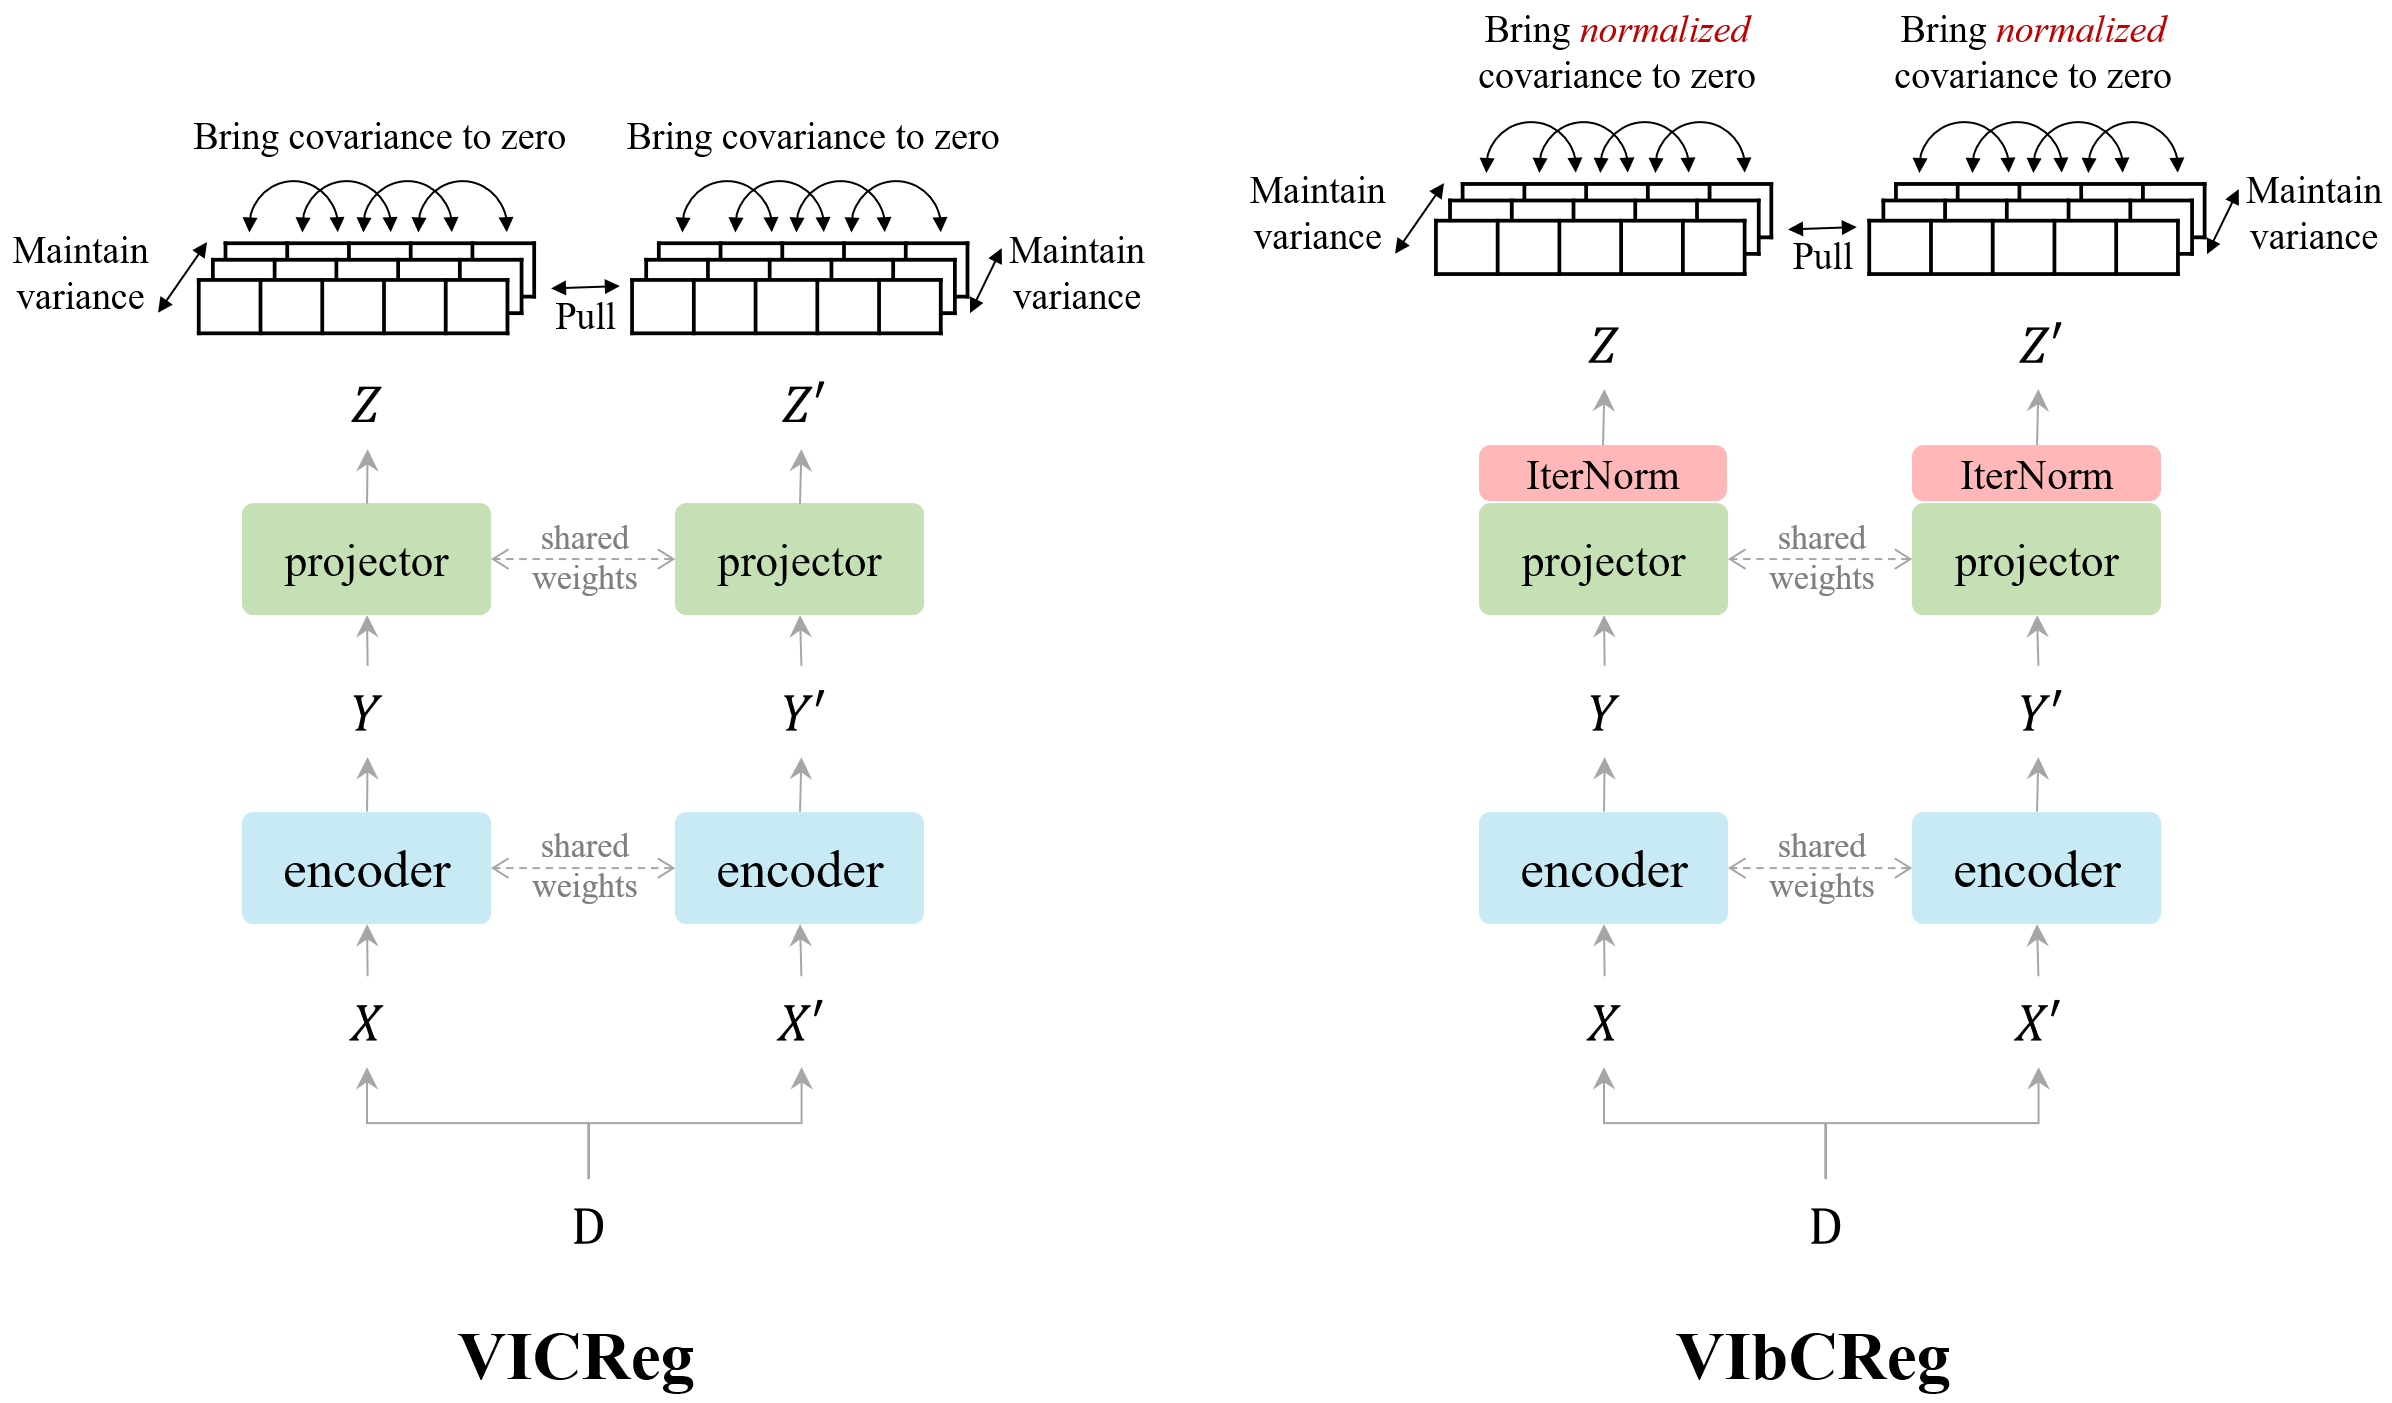
\includegraphics[scale=0.15]{VICReg_VIbCReg.png}
    \centering    
    \caption{\cite{lee2024vibcreg}}
\end{figure}




\end{document}